\begin{ex}
  No início de sua próxima aventura, Jones se defrontará com um terrível obstáculo. A probabilidade de que Jones passe por este obstáculo, saindo em boas condições físicas e mentais é 0,2; a de que saia em más condições é 0,5, e a de que não saia com vida é 0,3. Se conseguir vencer este obstáculo, encontrará outro logo a seguir. Neste novo obstáculo, a probabilidade de Jones sobreviver é 0,5, isto se chegar a ele em boas condições; mas esta possibilidade cai para 0,3 se Jones vier a enfrentá-lo em más condições. Qual é a probabilidade de que Jones sobreviva a estes dois obstáculos?
    \begin{enumerate}[(a)]
    \item 56\%
    \item 70\%
    \item 25\%
    \item 75\%
    \item 17\%
    \end{enumerate}
      \begin{sol}
       resposta: c  \\  \\
       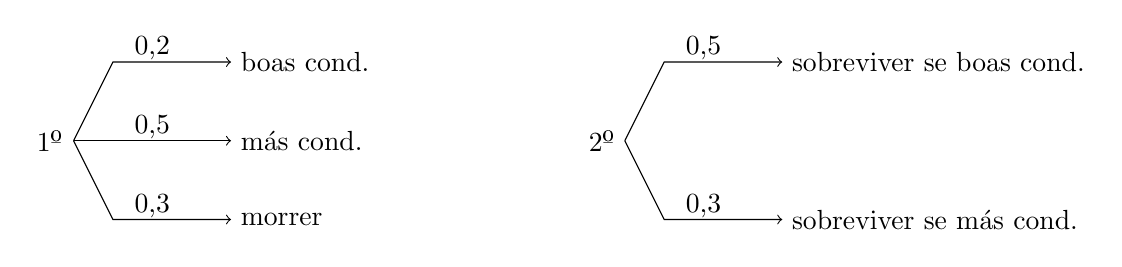
\begin{tikzpicture}
       \draw[->](0,0)--(0.5,1)--(2,1);\node at(-0.3,0){1º};\draw[->](0,0)--(0.5,-1)--(2,-1);
       \draw[->](0,0)--(2,0);\node at (1,0.9)[above]{0,2};
       \node at (1,-0.1)[above]{0,5};\node at (1,-1.1)[above]{0,3};\node at (2,1) [right]{boas cond.};\node at(2,0)[right]{más cond.};\node at(2,-1)[right]{morrer};
       \draw[->](7,0)--(7.5,1)--(9,1);\draw[->](7,0)--(7.5,-1)--(9,-1);\node at (7,0) [left]{2º};\node at (8,0.9) [above]{0,5};\node at(8,-1.1) [above]{0,3};\node at (9,1) [right]{sobreviver se boas cond.}; \node at (9,-1)[right]{sobreviver se más cond.}      ; \end{tikzpicture} 
       \\
       $\Rightarrow0,2\cdot0,5+0,5\cdot0,3=0,25=25\%$
      \end{sol}
\end{ex}